\newpage
\subsection{Textual; emptying}
\texHeader
\hypertarget{emptyPartition tex}{}

\texttt{}
\emph{}

\begin{itemize}
 
\item[$\blacktriangleright$] To initialize your control flow, you can take advantage of eMolfon's type completion here. Inside the \texttt{empty}
declaration, press  \texttt{control + space} to bring up a small context menu. Select \texttt{forEach} to write the pattern syntax
(Fig.~\ref{fig:typeCompletion}).

\vspace{0.5cm}

\begin{figure}[htpb]
\begin{center}
  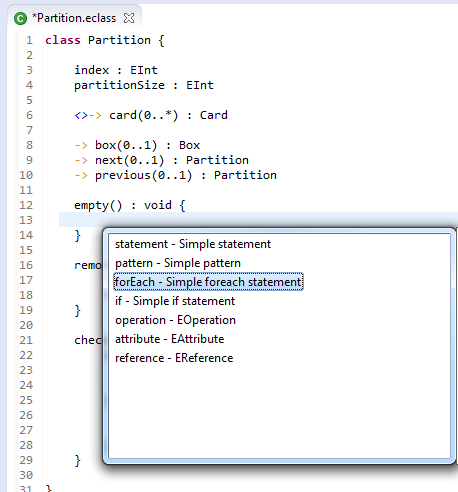
\includegraphics[width=0.7\textwidth]{eclipse_emptyTypeCompletion}
  \caption{eMoflon's Type Completion}
  \label{fig:typeCompletion}
\end{center}
\end{figure}

\vspace{0.5cm}

\item[$\blacktriangleright$] Create a single \texttt{deleteCardsInPartition}. Remove the second pattern automatically created since, for every card you delete,
you want to return to the loop and keep deleting for every match the pattern makes.

\vspace{0.5cm}

\item[$\blacktriangleright$] Your control flow should now resemble Fig.~\ref{fig:emptyControlFlow}

\clearpage

\begin{figure}[htpb]
\begin{center}
  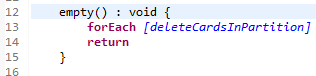
\includegraphics[width=0.5\textwidth]{eclipse_emptyControlFlow}
  \caption{Control flow for \texttt{empty}}
  \label{fig:emptyControlFlow}
\end{center}
\end{figure}

\item[$\blacktriangleright$] While similar to \texttt{removeCard}, this new pattern goes one step further by requesting a full destruction of card, instead of
just detaching the link. This means, in addition to destroying the link in \texttt{@this}, we need a destructive object variable. You can declare this special
type by prefacing \texttt{card} with an `-~-' operator.

\vspace{0.5cm}

\item[$\blacktriangleright$] Your workspace should now resemble Fig.~\ref{fig:emptyPattern}.

\vspace{0.5cm}

\begin{figure}[htpb]
\begin{center}
  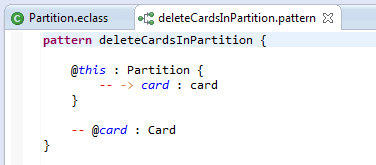
\includegraphics[width=0.6\textwidth]{eclipse_emptyPattern}
  \caption{Destroy an entire card, not just the link to it}
  \label{fig:emptyPattern}
\end{center}
\end{figure}

\item[$\blacktriangleright$] That's it - you're just speeding through these SDMs now! To see how it's done in the visual syntax, review Fig.~\ref{fig:sdm_end}
in the previous section.

\end{itemize}
